\chapter{Computational tools}
\label{compute}
In this Chapter an introduction to the tools used to for computations of both stellar evolution models and pulsation frequencies is provided. In \secref{sec:mesa}, the stellar structure and evolution code \texttt{MESA} is introduced, and the most relevant aspects for this work is discussed.  

\section{MESA}
\label{sec:mesa}

Modules for Experiments in Stellar Astrophysics or MESA is a suite of open source libraries that can be used to compute various applications in stellar astrophysics. Documentation can be found on the webpage \url{http://mesa.sourceforge.net/index.html} and from papers released with new updates \citep{paxton2010, paxton2013modules, paxton2015modules, paxton2018modules, paxton2019modules}.
MESA consists of several modules that works together in order to create computational models of stellar astrophysics. They have both the ability to work independently and each is constructed as a separate Fortran 95 library. All original modules \citep{paxton2010} with their purposes are listed in \tabref{modules}. 

\begin{table}[htbp]
\makebox[\textwidth]{
\begin{tabular}{lll}
\hline
\multicolumn{1}{l}{Name} & Type & \multicolumn{1}{l}{Purpose} \\ \hline
\texttt{alert}              & Utility          &    Error handling                          \\
\texttt{atm}                & Microphysics     &    Gray and non-gray atmospheres; tables and integration   \\
\texttt{const}              & Utility          &    Numerical and physical constants                      \\
\texttt{chem}               & Microphysics     &    Properties of elements and isotopes               \\
\texttt{diffusion}          & Macrophysics     &    Gravitational settling and chemical and  thermal diffusion\\
\texttt{eos}                & Microphysics     &    Equation of state                          \\
\texttt{interp\_1d}         & Numerics         &    One-dimensional interpolation routines    \\
\texttt{interp\_2d}         & Numerics         &    Two-dimensional interpolation routines            \\
\texttt{ionization}         & Microphysics     &    Average ionic charges for diffusion     \\
\texttt{jina}               & Macrophysics     &    Large nuclear reaction nets using reaclib           \\
\texttt{kap}                & Microphysics     &    Opacities                          \\
\texttt{karo}               & Microphysics     &    Alternative low-T opacities for C and N enhanced material  \\
\texttt{mlt}                & Macrophysics     &    Mixing length theory                          \\
\texttt{mtx}                & Numerics         &    Linear algebra matrix solvers                      \\
\texttt{net}                & Macrophysics     &    Small nuclear reaction nets optimized for performance   \\
\texttt{neu}                & Microphysics     &    Thermal neutrino rates                          \\
\texttt{num}                & Numerics         &    Solvers for ordinary differential and differential-algebraic equations\\
\texttt{package\_template}  & Utility          &    Template for making a new MESA-module            \\
\texttt{rates}              & Microphysics     &    Nuclear reaction rates                          \\
\texttt{screen}             & Microphysics     &    Nuclear reaction screening                          \\
\texttt{star}               & Evolution        &    One-dimensional stellar evolution                          \\
\texttt{utils}              & Utility          &    Miscellaneous utilities                          \\ 
\texttt{weaklib}            & Microphysics     &    Rates for weak nuclear reactions                        \\ \hline
\end{tabular}
}
\caption{MESA module Definitions and Purposes. From \citep{paxton2010}.}
\label{modules}
\end{table}
 
Here, the main focus will be on the \texttt{MESA star} 1D stellar evolution module. 

There are several modules that provides numerical methods used for the computations, the first being the  \texttt{mtx} module, providing an interface for linear algebra and matrix manipulation. The \texttt{num} uses these matrix routines as well as providing a number of solvers for ordinary differential equations from \citet{wanner1996solving}. It also includes a Newton-Raphson solver for multidimensional, nonlinear root finding (derived from Lesaffre's version of the Eggleton stellar evolution code \citep{eggleton1971evolution, pols1995approximate, lesaffre2006c}. The modules \texttt{interp\_1d} and \texttt{interp\_2d} uses 1-dimensional and 2-dimensional interpolation, respectively. Lastly, the \texttt{alert} module reports messages and errors and the \texttt{utils} module checks the variables for bad numbers such as NaN and infinity. 

\subsection{Stellar structure and evolution}

The \texttt{MESA star} module that implements several numerics and astrophysics modules to compute stellar evolution tracks using a Henyey-style code \citep{henyey1959method} with automatic mesh refinement, analytical Jacobians and solutions to coupled stellar structure and composition equations. The \texttt{MESA star} implementation is constructed with inspiration from stellar evolution and hydrodynamics codes such as EV \citep{eggleton1971evolution}, EVOL \citep{herwig2004evolution}, EZ \citep{paxton2004ez}, FLASH-the-tortoise \citep{lesaffre2006c}, GARSTEC \citep{weiss2008garstec}, NOVA \citep{starrfield2000effects}, TITAN \citep{gehmeyr1994adaptive} and TYCHO \citep{young2005observational}.

Firstly, \texttt{MESA star} reads the input files needed for the run. There are two files that determine the specific controls for \texttt{MESA star} to read and implement. The first file specifies the type of evolutionary calculation, EOS and opacity prescriptions, and chemical composition among other properties. Changing the parameters in this file allows to make a grid as described in \secref{sec:grid}. The second file specifies the controls to be applied during the run
All of the options for the inlist files can be found in the documentation. There are generally two ways to initiate an evolutionary run. One option is to let \texttt{MESA} evolve a PMS model based on an input of an input mass, luminosity and initial abundances. The star then evolves from the PMS and until a certain stop criterion is fulfilled. However, if an entire grid is needed it is a disadvantage to calculate all the PMS models for all individual tracks. The second (and more favorable) option in this work, is to use a pre-calculated PMS model in the inlist and let \texttt{MESA} relax the parameters in the following evolution. In this work a 1.7\msun PMS model is applied for this purpose \footnote{However, one needs to be aware that relaxing the parameters can give numerical issues if the PMS sequence model and the initial parameters used for further evolution are too far apart (since it would be numerically feasibly to relax the mass of a 1.7\msun model to 8\msun).}. %However, the grid calculated in this work (see \secref{sec:grid}) combined with the 1.7\msun PMS sequence model only poses numerical issues for a few tracks, see \secref{sec:grid}. 

When the input files have been read, the physics modules (EOS, opacities and nuclear network) are initialized. In the first step, the evolutionary run begins. \texttt{MESA} then continues the evolution by continuing to the next time step. As this happens, the model is remeshed if nescessary, mass loss is taken into account (although not used in this work since the mass is assumed constant after being relaxed to the MS), abundances are adjusted by taken diffusion into account, and the solvers are called (Newton-Rapshon) to calculate a new structure and composition solution. Lastly, a new time step is calculated. Within this one time step, \texttt{MESA star} builds a one-dimensional spherically symmetric model, where the star is divided into cells reaching from the core to the surface of the star. During one time step, \texttt{MESA} does not solve structure equations separately from composition equations. Instead, an entire set of coupled equations are solved for all cells simultaneously. Some of the controls for adjusting structure and time steps relevant for this work are further discussed in \secref{sec:res}.

\subsection{Output}
There are three different types of output files in \texttt{MESA}, which can be used for different purposes. The first is the \textit{history} file, where the history for the entire run is saved. The header contains information on the initial parameters set in the run such as the initial mass and Z abundance. Hereafter, one line corresponds to one \textit{model}. The first two columns contain information on the \textit{model\_number}. The rest of the columns show calculated properties such as age, mass and luminosity. 

The next output file is the \textit{profile}. On the contrary to the history files, the profiles only contain information of one model. The first line shows the global properties such as the age. The rest of the file shows properties for each point or \textit{zone} in the model. Since it is computationally heavy for \texttt{MESA} to write the profiles, it is necessary to evaluate whether all zones are needed in the output files. For this project, it was found sufficient to only use information on the core and surface. 

The third output file is \textit{profiles.index}. Since \texttt{MESA} does not save profiles for every \textit{step}, the \textit{profile number} and model number are not necessarily the same. Therefore, the profiles.index tells the user how to translate between these.

Additionally, in order to be able to calculate the frequencies in GYRE, an output file for this is needed. This is done by adding the \texttt{write\_pulse\_data\_with\_profile = .true.} command to the the inlist, producing a \textit{profile.GYRE} file for each corresponding profile. These will be described in more detail in \secref{sec:gyre}.


\subsection{Convection treatment}
\label{sec:conv_prescriptions}

In \secref{sec:energybyconvection} the condition for convection has already been discussed briefly. There are several theories that leads to a numerical implementation.  Therefore, the main focus here will be the implementation of \texttt{MESA mlt} module. 

The implementation of convection in both \texttt{MESA} and the Warsaw-New Jersey stellar evolution code is based on the standard-mixing length theory of convection as presented by \citet{weiss2004cox}. This theory provides a very simplified picture of the physical processes of convection, as well as a qualitative and reasonable description of heat transfer by convection. However, the quantitative results should not be expected to have high accuracy or reliability. One parameter that particularly causes discussions due to its high uncertainty, is the parameter describing the mixing length itself. The mixing length, $\Lambda$ is described as the mean-free path that a fluid element travels inside a convectively unstable region in a star. In outer layers of a star, it can be assumed that $\Lambda$ is proportional to the pressure scale height $\lambda_p$. In \texttt{MESA mlt}, the mixing-length is therefore implemented as
%
\begin{equation}
    \Lambda \equiv \alpha_{mlt} \lambda_p,
\end{equation}
%
where $\alpha_{mlt}$ is the parameter input in \texttt{MESA}. It is generally assumed to be constant throughout the star. The value of this parameter is only known to be of order one (while the default value in \texttt{MESA} is 2), from physical arguments. Having a high mixing length in outer layers essentially means that the bubbles can travel far before dissolving into the environment and the convection is efficient. For $\delta$ Sct stars, the convective outer layer is significantly smaller than that of solar-type stars. Therefore, it is safe to assume smaller efficienty of energy transport by convection. On \figref{mlt}, evolutionary tracks for two models with different mass can be seen in an HR-diagram. The black line shows the track calculated with  $\alpha_{mlt}= 0.2$ and the red with $\alpha_{mlt}= 0.8$. From this it is clear that the dependence on the mixing-length parameter is not very significant until just before the red giant branch. Here, the higher $\alpha_{mlt}$ causes a significant drop in luminosity, due to the vast changes in the structure. %This is because the convective layer of the star deepens as it moves closer towards the red giant branch, meaning that energy transport by convection dominates over radiation. A higher value of $\alpha_{mlt}$ thereby has a larger effect at this stage as it causes an increase in convective efficiency (hence a decrease in energy transport by radiation) and a drop in luminosity. 


\begin{figure}[htbp]
    \centering
    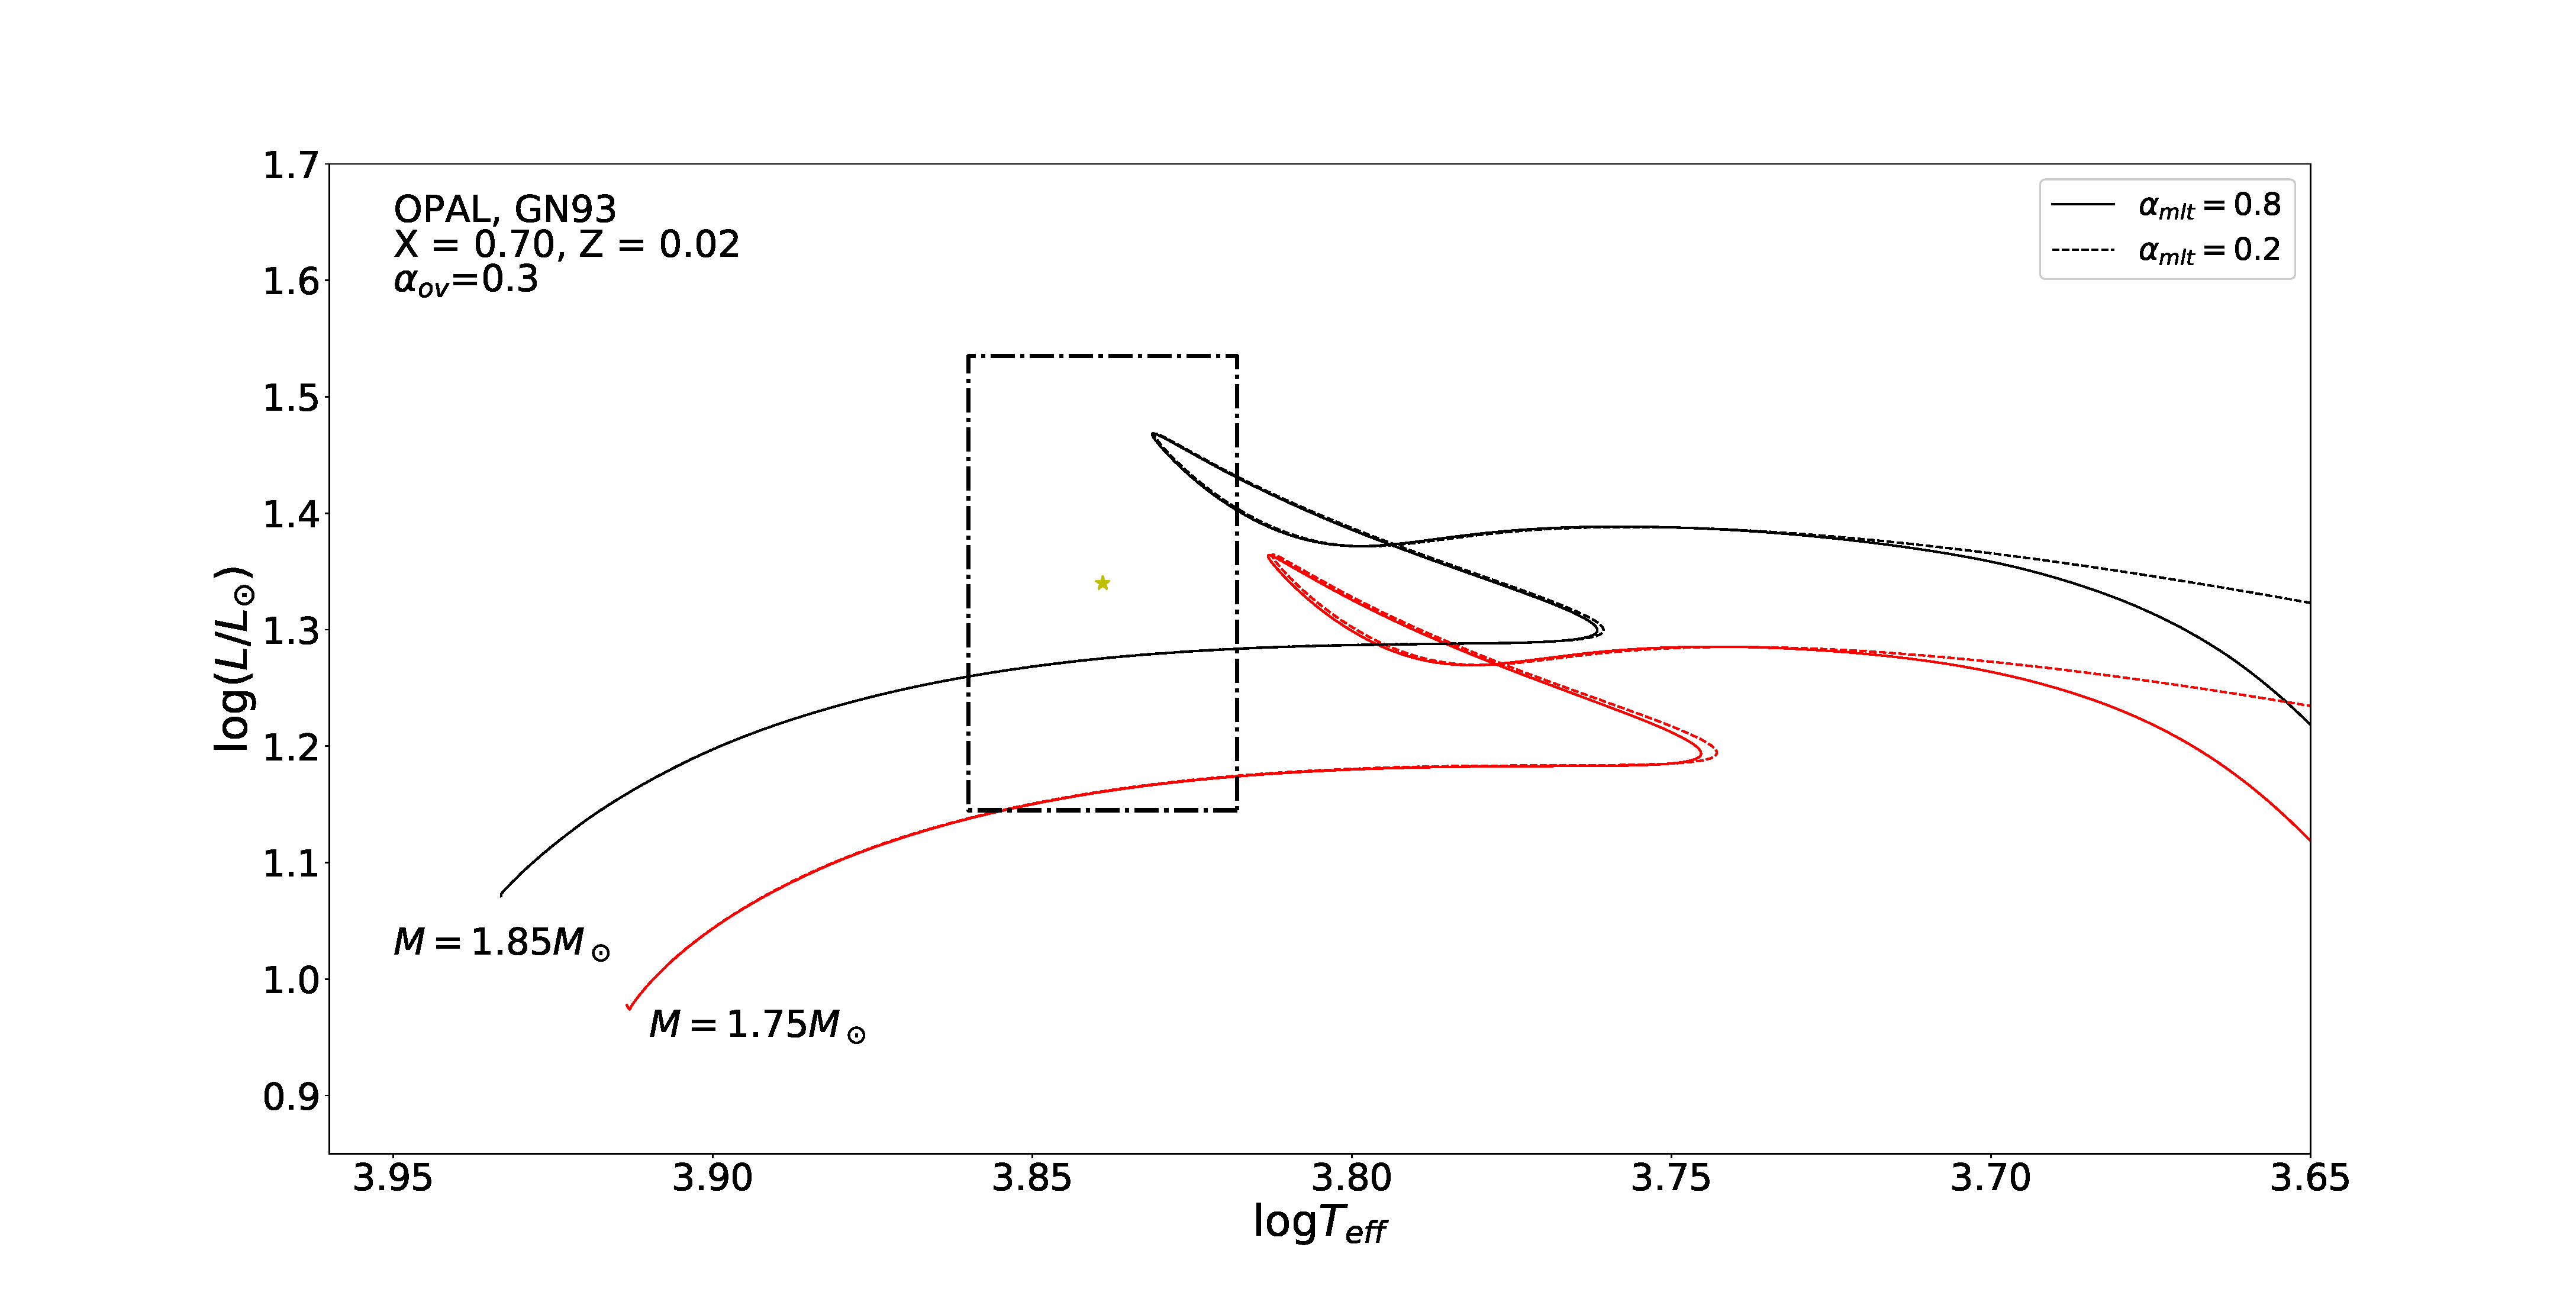
\includegraphics[width=1\textwidth]{mlt.eps}
    \caption{Evolutionary tracks with masses of $M=1.75$\msun and $1.85$\msun and parameter combinations of $X=0.70$,$Z=0.02$, $\alpha_{ov}=0.2$. Each are calcululated with two different mixing lengths of $\alpha_{mlt}=0.5$ (red line) and $\alpha_{mlt}=0.5$ (black line). The black dashed line indicates errobox for uncertainties for observed parameters from \citet{lenz2010delta}.}
    \label{mlt}
\end{figure}

Even though the mixing length paints a nice picture of the convection in the outer layers, there are still issues related to the convection deep in the interior. Specifically to which extend chemical elements are mixed, as it has a big impact on the later evolution of the star. For MS stars with a convective cores the main discussion topic is the convective core overshooting. The convective core overshooting relates to the issue that the boundary between convective core and radiative layers is not sharp; instead, the convection "overshoots" into the layer above (for a quantitative description, see \citet{kippenhahn1990stellar}, Chap. 30). The amount of overshoot depends on the velocity of the convective elements and the breaking force, which are difficult to find as it includes non-local solutions to velocities, gradients and fluxes in the entire core. Therefore, the values for overshooting are, as for the mixing length), arbitrary and can only be evaluated through modeling. 

There are two standard methods that are commonly used to calculate the overshoot numerically. The first one is quite similar to that of the mixing length, describing the extension of the convective region defined by the Schwarzschild criterion, in terms of pressure scale height

\begin{equation}
    l_{ov} = \alpha_{ov}H_p,  
\end{equation}

\noindent in which $\alpha_{ov}$ is typically in the order of 0.1 and 0.2. Even though it resembles the description of the mixing length parameter $\alpha_{mlt}$, it has no relation to it and is purely detemined through comparing models to observations. This prescription is applied as "step overshoot" in MESA. The second method considers convective overshoot as a diffusive process with a diffusion constant depending on the radial distance z from the border defined from the Schwarzschild criterion. 

\begin{equation}
    D(z) = D_0 \exp{\frac{-2z}{f_{ov}H_p}},
\end{equation}

\noindent where $f_{ov}$ is a free parameter in the order of 0.02, and $D_0$ sets the scale of the diffusive speed. This prescription has a particular advantage as it can be added quite easily to a stellar evolution code where diffusion is already implemented. However, for this work, only the former prescription is implemented.

The reason that convective core overshoot is important to implement is that the overshoot causes additional mixing of elements. Hence, more hydrogen is transported to the core, acting as additional fuel on the main sequence. Therefore, just a small extension to the convective core causes a significant continuastion of the main sequence. An example can be seen on \figref{ov_example}, where two stellar evolution tracks of masses 1.95\msun and 1.75\msun are shown. The black line indicates a track with $\alpha_{ov}=0.2$ and the red line the corresponding track with $\alpha_{ov}=0.3$. it can here clearly be seen that the main sequence is significantly longer for models with higher $\alpha_{ov}$, and that it affects the remaining part of the evolution as well. 

\begin{figure}[htbp]
    \centering
    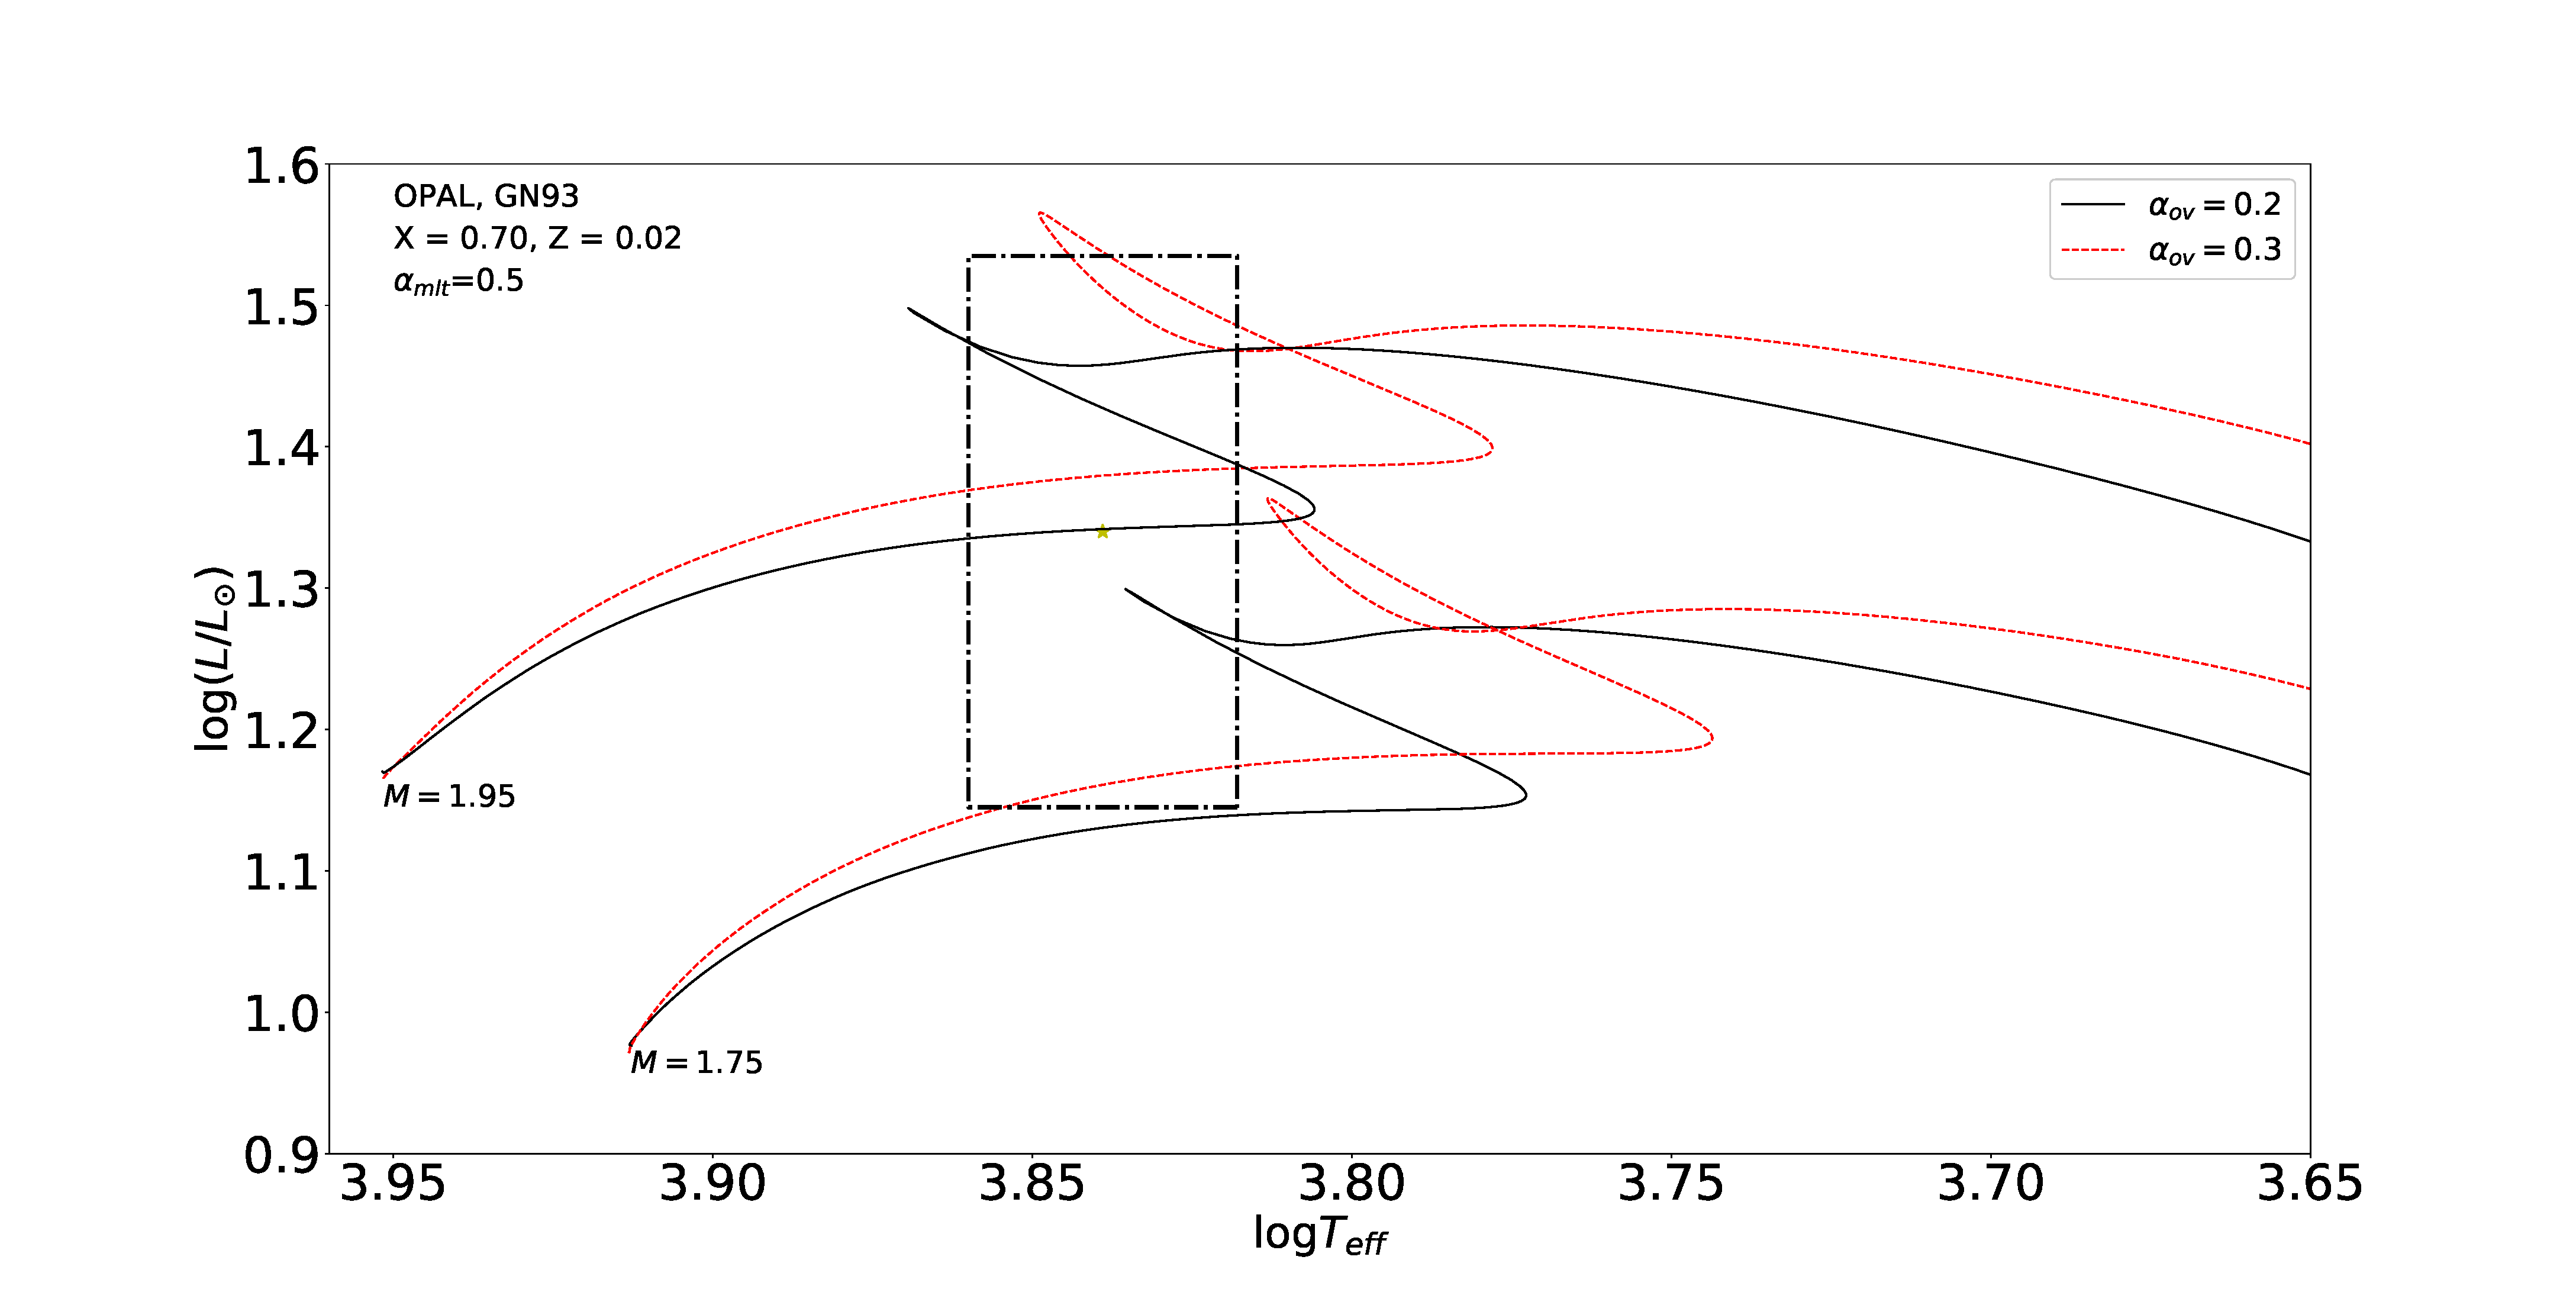
\includegraphics[width=1\textwidth]{overshoots_example.eps}
    \caption{Evolutionary tracks with masses of $M=1.75$\msun and $1.85$\msun and parameter combinations of $X=0.70$,$Z=0.02$, $\alpha_{mlt}=0.5$. Each are calcululated with two different mixing lengths of $\alpha_{ov}=0.3$ (red line) and $\alpha_{ov}=0.2$ (black line). The black dashed line indicates errobox for uncertainties for observed parameters from \citet{lenz2010delta}}
    \label{ov_example}
\end{figure}
\subsection{Element abundance mixtures}

In order for \texttt{MESA} to calculate a stellar model, the element abundances needs to be implemented. The chemical composition of a star is assumed to be a reflection of the distribution of elements in the cloud from which the star was born, assuming that the composition is preserved in the outer layer of the star. %Photospheric observations have revealed that abundance patterns of regular $\delta$ Sct stars are similar to those of the solar neighbourhood \citep{}
Since solar neighbourhood abundances are usually more accurately measured than stars outside, the solar element mixture is commonly used for modeling stars from outside the neighbourhood as well. In MESA, the initial abundances X (hydrogen), Y (helium) and Z (metals, i.e. all elements with atomic numbers higher than helium) is given in terms of mass fractions where $1=X+Y+Z$ must always be fulfilled. 

The solar element abundances depends on the choice of theoretical atmosphere model. Hence, they are updated continuously as atmosphere models are changed and improved. There are several abbreviations of element mixtures that can be appliued in \texttt{MESA}, such as GN93 \citep{grevesse1993cosmic}, GS98 \citep{grevesse1998standard} and a09 \citep{asplund2009chemical}. %The most commonly used solar element abundances are GN93. The solar mass fractions for thise abbreviations are given in \tabref{tab:solar}
\citet{grevesse1993cosmic} used a one-dimensional hydrostatic atmosphere model to derive the solar abundances, and compared to the solar system abundances extracted from meteorites, and found good agreement. This is what is used in this project. The main reason for this is that compared to a09, GN93 does not have issues such as \textit{the solar abundance problem}\citep{asplund2009chemical}. The importance of element mixture choice is further discussed in \secref{sec:discussion}. 

\subsection{Equation of state}

The equation of state takes the density and temperature and calculate the corresponding pressure, ionization degrees and thermodynamic quantities necessary to calculate the stellar structure. 

The equation of state is implemented through the \texttt{EOS} module, where density $\rho$ and temperature $T$ are treated as independent variables in the Helmholtz free energy formulation. However, some calculations are carried out through the Gibbs free energy formulation where the density can be provided through root-finding. This is computationally heavy, so the roots are therefore pre-processed, creating $P_{gas}$ and $T$ tables that allows for a quicker solution when calling the \texttt{EOS} module (provided that the input values are within the range of the pre-computed values). The $\rho-T$ tables are based on OPAL EOS tables from \citet{rogers2002updated}, and for lower values \citet{saumon1995equation}, covering an area up to $Z \leqslant 0.04$. If parameters are outside of the region covered by the \texttt{MESA} tables, the EOS from HELM \citep{timmes2000accuracy} and PC \citep{potekhin2010thermodynamic} are used. These use a free energy approach assuming complete ionization, which is applicable to the region outside of the tables (where cooler stars are only partly ionized). 

\subsection{Opacity data}

From the density, temperature and chemical composition, the EOS yields estimates on the ionization equilibrium concentrations and level populations in a medium. These can be used to evaluate the Rosseland mean opacities. These are implemented though the \texttt{kap} module in \texttt{MESA}, where pre-processed opacity tables are within the \texttt{make\_kap} module. The electron conduction opacity
tables are based on \citet{cassisi2007updated}. For the radiative opcaities, low temperature regions ($\log T \leqslant 4$) is covered by \citet{freedman2008line} or \citet{ferguson2005low}.

Radiative opacities have been calculated by two teams, OPAL and OP. The references for the groups are listed in \tabref{opaci}

\begin{table}
	\centering
	\caption{References for the two opacity groups.}
	\label{opaci}
	\begin{tabular}{ll}
		\toprule
		Source               & Reference \\
		\midrule
		OPAL                 &   \citet{iglesias1996updated}        \\
		OP (Opacity Project) &  \citet{badnell2005updated}       \\ 
		\bottomrule
	\end{tabular}
\end{table} 

Both groups uses slightly different methods to compute the radiative opacities \citep{seaton2004comparison}. For this project, only the OPAL opacities are implemented, which will be discussed briefly in \chapref{sec:discussion}. 
\section{GYRE}
\label{sec:gyre}

In order to interpret asteroseismic observations from recent mission such as MOST \citep{walker2003most,matthews2007one}, CoRot \citep{michel2008first} and Kepler \citep{borucki2009transiting, gilliland2010kepler}, a stellar oscillation code calculating
the eigenfrequency spectrum of an input stellar model is needed. 
The asteroseismic module included in \texttt{MESA} is based on the stellar pulsation code \texttt{ADIPLS} \citep{christensen2008adipls}, which allows for a calculation of the eigenfrecuencies. However, a demand for more detailed non-adiabatic calculations lead to the development of \texttt{GYRE}, which is an open source pulsation code from 2013 described in  \citep{townsend2013, townsend2017} and on the webpage \citep{bitgyre}. 

\texttt{GYRE} is written in \texttt{Fortran 2008} and uses a \textit{Magnus Multiple Shooting} (MMS) scheme to solve linearized pulsation equations. The following steps are used to calculate the eigenfrequencies for an arbitrary input model:

\begin{enumerate}
    \item \emph{Stellar model} As a first step, \texttt{GYRE} needs to read an input model. This model can be either read from a pre-built or can be constructed analytically. It supports three different classes of models. The first is the evolutionary models (which is what is used in this work) constructed from a stellar evolution code. The second relies on polytropic models, and the last is purely analytical calculations based on explicit expressions for structure coefficients. 
    \item \emph{Grid calculation} When the file has been read, a calculation grid is constructed. The grid allows for multiple shooting and eigenfunction reconstruction. The type of grid idepends on the type of input model. 
    \item \emph{Root-finding} Initial guesses for discriminant roots are found by scanning the frequency space in the grid. 
    \item \emph{Eigenfunctions} Based on the initial guesses of roots, the corresponding eigenfunctions are then constructed. 
\end{enumerate}

These are only the very basic steps used by \texttt{GYRE}; a more detailed description of the numerical steps used is beyond the scope of this work, and the reader is instead referred to \citep{townsend2013}.

It is now also possible for \texttt{GYRE} to be implemented directly in the \texttt{MESA star} module, which couples calculations of both stellar evolution and frequencies. However, implementing it is a bit more intricate than reading in the files separately; therefore, the first method is used in this project (calculating a grid of models that can then be used as an input for the \texttt{GYRE} calculations). 

\subsection{Input and output options}

\texttt{GYRE} reads input parameters given in an input file. The input file is structured in a similar way as the \texttt{MESA} inlist files, consisting of several namelist groups: 

\begin{itemize}
    \item \emph{Constants} Defines the physical constants such as the gravitational constant and solar parameters (mass, luminosity etc.)
    \item \emph{Stellar model} Defines the stellar model that \texttt{GYRE} reads and constructs eigenfrequencies for. 
    \item \emph{Mode parameters} Defines mode parameters such as $l,m$ and minimum and maximum radial orders. 
    \item \emph{Oscillation parameters} Defines the parameters relates to the oscillation, such as inner and outer voundary conditions and rotation. 
    \item \emph{Numerical parameters} Specifies numerical methods parameters. 
    \item \emph{Frequency scan} Defines the span of the frequency space scan with a set of points. 
    \item \emph{Calculation grid} Defines the parameters used for the calculation grid. 
    \item \emph{Output files} Specifies the output produced by the end of a run. This includes the file format, frequency units, comma separation etc.  
\end{itemize}

For this project, the input model is constructed as a .GYRE file for every profile constructed in \texttt{MESA}, which is then read into the \texttt{GYRE} input file. The input files used in this project for 44 Tau and Superstar is constructed from a bash script which can be seen in \secref{inlist}. When the input file has successfully been read and the calculations have finished, \texttt{GYRE} constructs one of two different types of ouput files. The first is the Summary files that provides global information on the theoretically produced modes. The second is the mode files, containing information on a single mode including detailed eigenfunction quantities such as rotation kernels. For this project, the first file is used. The contents of the output file is defined in the input file described above with the \texttt{summary\_item\_list} (or, correspondingly \texttt{mode\_item\_list}). The most relevant for this project is the harmonic degree, radial order and frequencies. Options for non-adiabaticity can be included in the \texttt{GYRE} calculations and will be discussed in \chapref{sec:discussion}.

%Several options for non-adiabaticity can be included in the \texttt{GYRE} calculations. This has the advantage that it yields the excited frequency range which can be compared to observations. One of the major contradictions between observations and theory in asteroseismology is that theory predicts all frequencies to be excited if the pulsations are driven by the kappa mechanism. But unfortunately, this is not what is observed, Therefore, using non-adiabatic calculations can provide a more detailed information on the excitation of each mode. However, the major disadvantage of this is that since non-adiabatic equations rely on solving non-linear equations, the calculation time increases significantly from that of adiabatic calculations. Especially if it needs to be done for an entire grid. Therefore, this option is not used in this work.  